\section{Redes Estocásticas}

\subsection{Definições}
\begin{frame}{Redes Estocásticas}%
  \justifying%
  Podemos considerar também o caso em que as unidades $\mathrm{x}_{i}$ de uma rede são variáveis aleatórias. É o que acontece numa rede Estocástica.
  \\~\\
  A unidade $\mathrm{x}_{i}$ tem agora certa probabilidade $P$ de ser encontrado com valor $x_{i} = 1$, e probabilidade $1 - P$, com valor $x_{i} = 0$.
\end{frame}

\begin{frame}{Função de Ativação}%
  \justifying%
  Outra forma para a função de ativação.
  \begin{figure}[h]{}%
    \label{fig:stoc-activation}%
    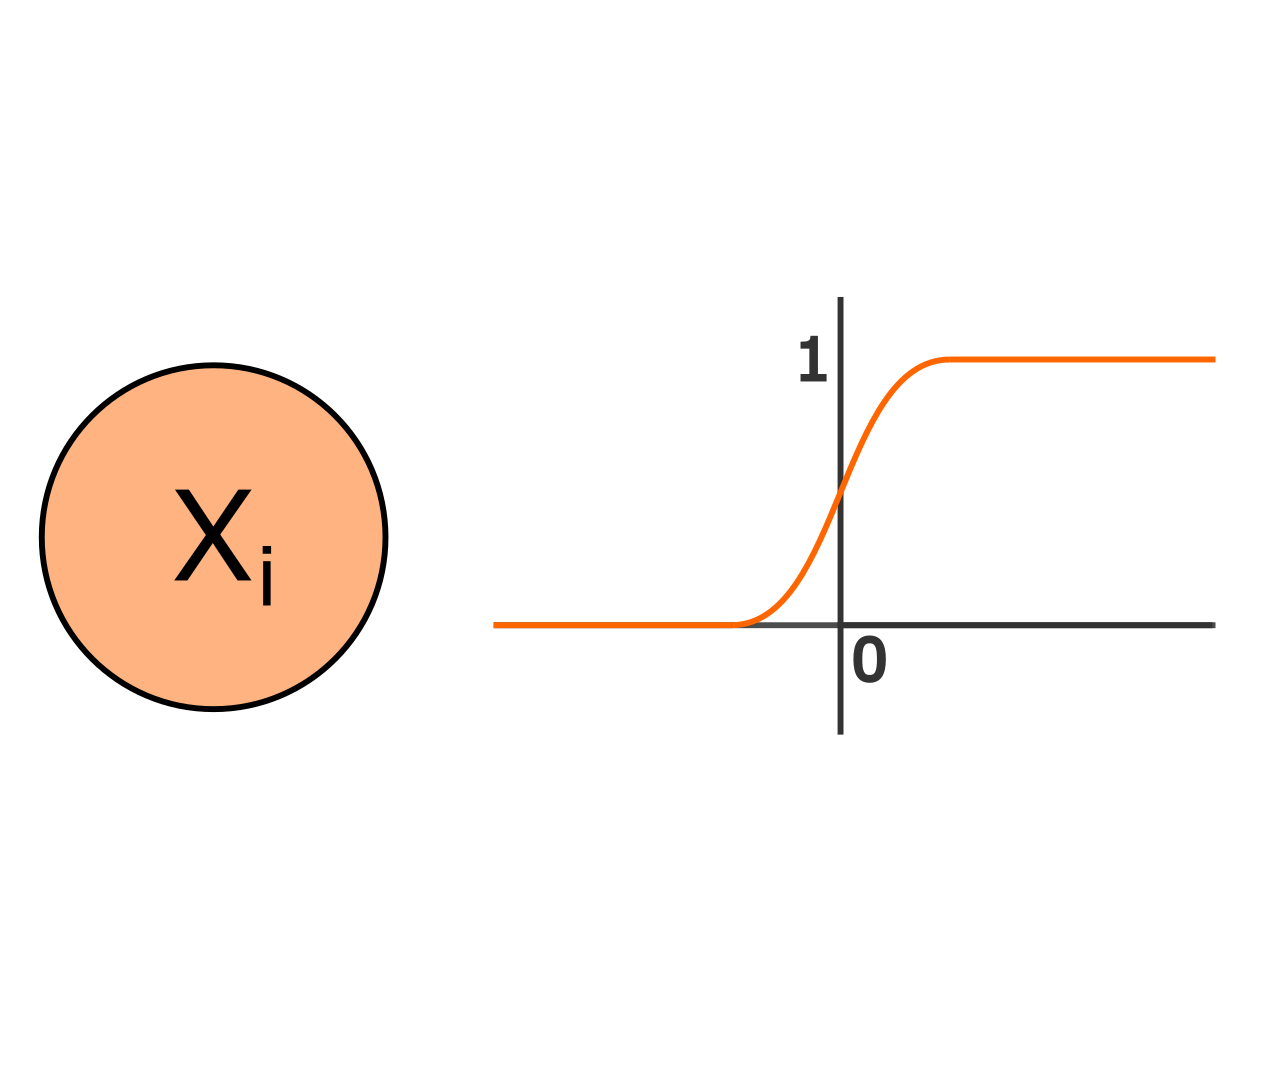
\includegraphics[scale=0.35]{images/stochastic_activation.png}
    \caption{Função de ativação de uma unidade na rede de Hopfield.}
  \end{figure}
\end{frame}

\begin{frame}{Função de Ativação}%
  \justifying%
  Função logística, ao invés de função degrau $\dots$
  \begin{equation}%
    \label{eq:stoc-prob}
    x_{i} = P(h_{i}) = \frac{1}{1 + e^{(-2\beta h_{i})}}
  \end{equation}
  \\~\\
  \begin{equation}%
    \label{eq:hi}%
    h_{i} = \sum_{j} \omega_{ij} x_{j}
  \end{equation}
\end{frame}

\begin{frame}{Temperatura -- Ruído}%
  \justifying%
  Na equação~(\ref{eq:stoc-prob}), temos o parâmetro $\beta$, que corresponde ao inverso da temperatura $T$.
  \\~\\
  Esta temperatura não tem o mesmo significado físico, mas é usado aqui para introduzir ruído. Controlar a inclinação da função logística.
  \\~\\
  Se $\beta$ for muito grande, ou seja, temperatura muito baixa, o sistema retorna à situação determinística. A função logística passa a ser a função degrau.
\end{frame}

\subsection{Esquema}
\begin{frame}{Rede Estocástica diagrama}%
  \begin{figure}%
    \label{fig:stoc-diagram}%
    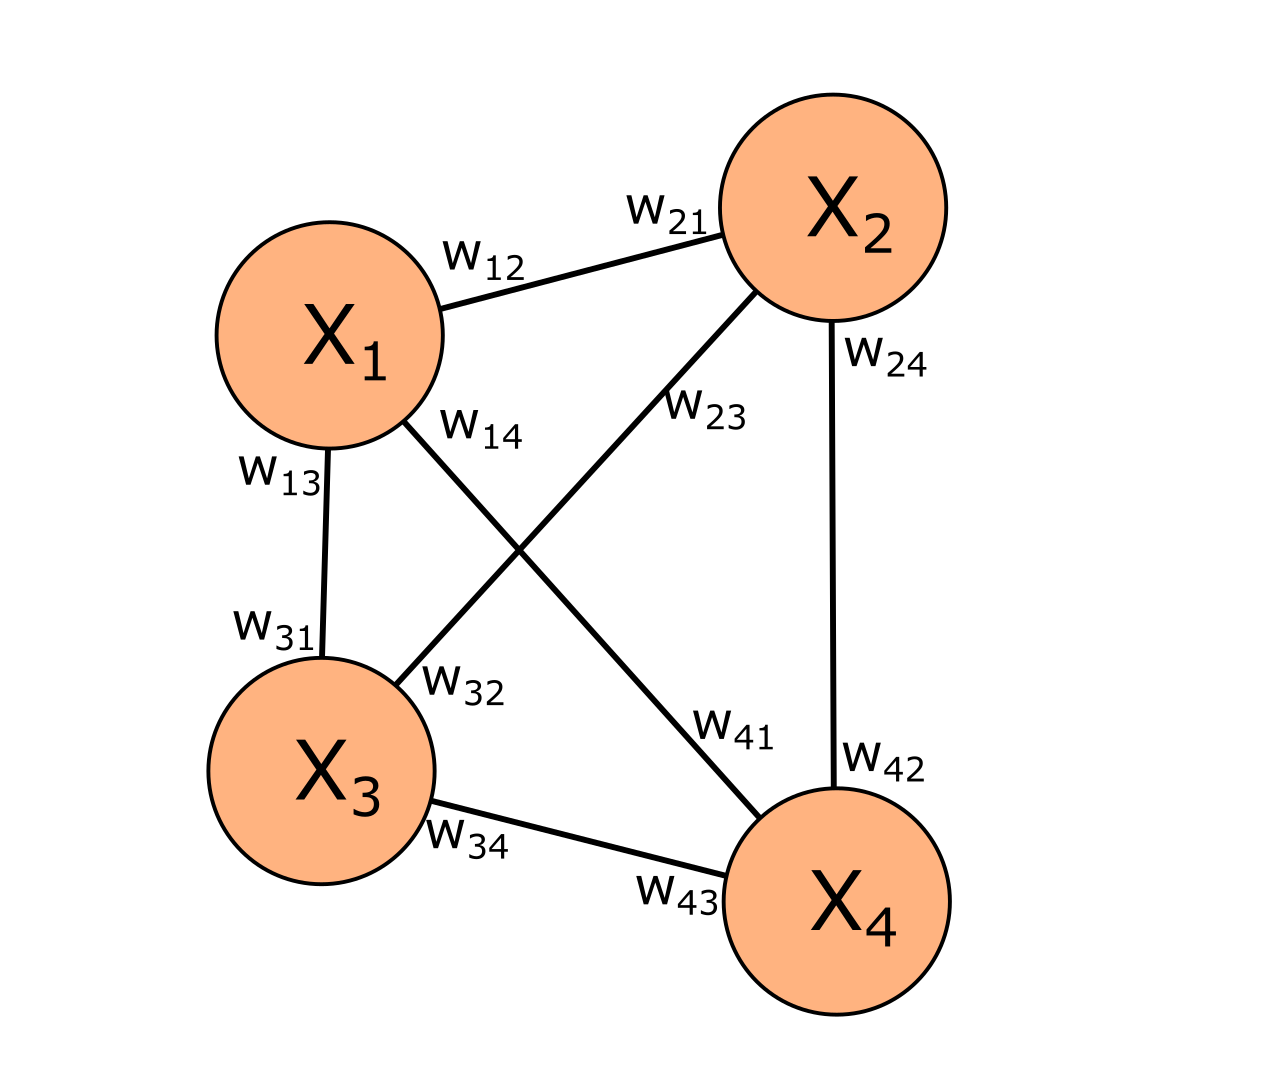
\includegraphics[scale=0.5]{images/stochastic_full.png}
    \caption{Rede estocástica com 4 unidades e suas respectivas conexões.}
  \end{figure}
\end{frame}

